\section{Reverb Implementation in Assembly}

The reverb implementation in Assembly was done by being inspired from the Matlab Code in \autoref{sec:rev_del}. The code is in the file \textit{reverb.asm}. In the following, each subsection will represent either a subroutine or a macro. 

\subsection{The \textit{reverb_pre} Subroutine}

Since the same buffer is used for all the effects and for different purposes in the same effect, the address of the buffer that contains the needed coefficients for this subroutine is set in the first two lines. The input is also moved to the \textit{X[N]} buffer. \\
This subroutine is destined to compute the first section of the reverb, the part just before the comb filter. This part is shown in figure \autoref{fig:pre_reverb_block_design}, a fraction of the whole effect diagram in figure \autoref{fig:reverb_block_design}. \\
The idea in the code is to point on different parts of AC0 which contains values of \textit{X[N-t]}, the more the pointer has a lower negative number, the bigger the delay. Different values at the pre-calculated delays \textit{ed1}, \textit{ed2}, \textit{ed3} and \textit{ed4} are added together to give $X_{1}[N]$ and then stored in AR5. \\

\begin{figure} [htbp]
 \centering
\begin{picture}(0,0)%
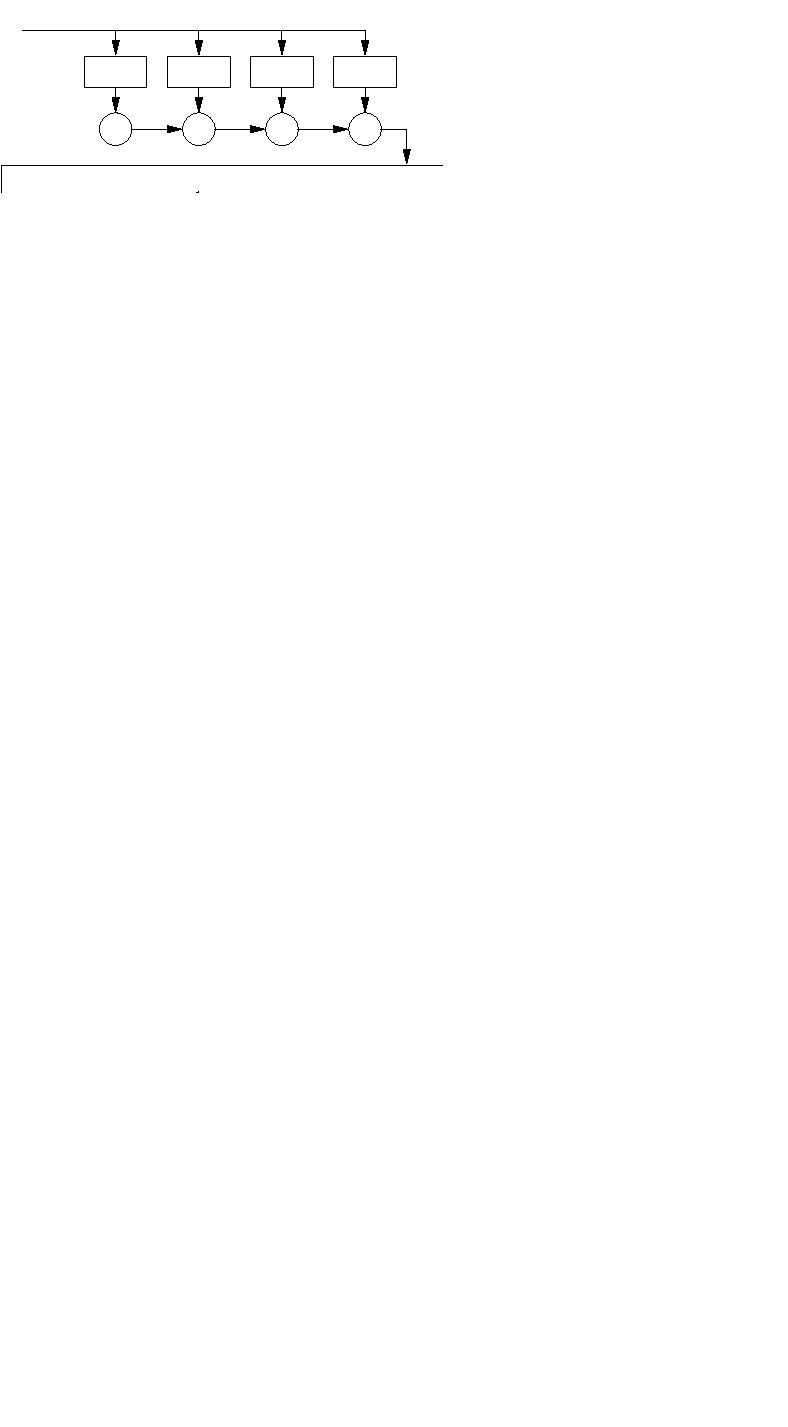
\includegraphics{pre_reverb_serial_des.pdf}%
\end{picture}%
\setlength{\unitlength}{3646sp}%
%
\begingroup\makeatletter\ifx\SetFigFont\undefined%
\gdef\SetFigFont#1#2#3#4#5{%
  \reset@font\fontsize{#1}{#2pt}%
  \fontfamily{#3}\fontseries{#4}\fontshape{#5}%
  \selectfont}%
\fi\endgroup%
\begin{picture}(5832,1599)(-1319,-1288)
\put(-314,4934){$x_1[n]$}%
\put(-3464,6419){$x[n]$}%
\put(-1439,5879){$z^{-ed_3}$}%
\put(-719,5879){$z^{-ed_4}$}%
\put(-2744,-1319){$\Sigma$}%
\put(-2024,-1319){$\Sigma$}%
\put(-1304,-1319){$\Sigma$}%
\put(-2159,-1319){$z^{-ed_2}$}%
\put(-2879,-1319){$z^{-ed_1}$}%
\put(-584,-1319){$\Sigma$}%
\end{picture}%
  \caption{Part of the Block diagram of a \gls{reverb} unit.}
  \label{fig:pre_reverb_block_design}
\end{figure}

\subsection{The \textit{reverb_lpcf} Subroutine}

This subroutine is responsible for computing the equations of the 6 comb filters. \\
The first part is reserved for calculating the different coefficients needed in the calculations like $LD$ and $f$. \\
The beginning of the macro command marks the end of coefficients calculations and the beginning of the equations processing. \\
The choice of a macro implementation here comes after observing big similarities between the six comb filters. The only differences lie in the $b_{i}$ gains, $x_{i}$ values and $d_{i}$ values. This is why they are macro entries. \\
The macro is simply the computation of the equations \ref{eq:reverb_eq_iir1w} to \ref{eq:reverb_eq_iir6w}. The circular buffer AR0 is the one that contains the values of $x_{i}$ and AR4 the one that contains the coefficients, gains and delay values. \\
After the macro section, it is called with the different comb filter settings in a row. 

\subsection{The \textit{reverb_allpass} Subroutine}

The subroutine is the one that takes into account the final part of the reverb effect which is the two all-pass filters. It also involves the use of a macro as the previous section since the two all-pass filters have considerable resemblance. \\
Again, AC0 is used as a buffer for the $x_{i}$ values and AR4 for the coefficients and the delay values. The other registers and accumulators are used for temporary purposes. \\
Last but not least, the data is moved to T2 that plays the role of the output. 
Another crucial step is to move the pointer of the AC0 buffer so that in the next iteration the values are not overwritten but inserted in a new slot. \\





